\documentclass[twoside]{book}

% Packages required by doxygen
\usepackage{fixltx2e}
\usepackage{calc}
\usepackage{doxygen}
\usepackage[export]{adjustbox} % also loads graphicx
\usepackage{graphicx}
\usepackage[utf8]{inputenc}
\usepackage{makeidx}
\usepackage{multicol}
\usepackage{multirow}
\PassOptionsToPackage{warn}{textcomp}
\usepackage{textcomp}
\usepackage[nointegrals]{wasysym}
\usepackage[table]{xcolor}

% NLS support packages
\usepackage{polski}
\usepackage[T1]{fontenc}

% Font selection
\usepackage[T1]{fontenc}
\usepackage[scaled=.90]{helvet}
\usepackage{courier}
\usepackage{amssymb}
\usepackage{sectsty}
\renewcommand{\familydefault}{\sfdefault}
\allsectionsfont{%
  \fontseries{bc}\selectfont%
  \color{darkgray}%
}
\renewcommand{\DoxyLabelFont}{%
  \fontseries{bc}\selectfont%
  \color{darkgray}%
}
\newcommand{\+}{\discretionary{\mbox{\scriptsize$\hookleftarrow$}}{}{}}

% Page & text layout
\usepackage{geometry}
\geometry{%
  a4paper,%
  top=2.5cm,%
  bottom=2.5cm,%
  left=2.5cm,%
  right=2.5cm%
}
\tolerance=750
\hfuzz=15pt
\hbadness=750
\setlength{\emergencystretch}{15pt}
\setlength{\parindent}{0cm}
\setlength{\parskip}{3ex plus 2ex minus 2ex}
\makeatletter
\renewcommand{\paragraph}{%
  \@startsection{paragraph}{4}{0ex}{-1.0ex}{1.0ex}{%
    \normalfont\normalsize\bfseries\SS@parafont%
  }%
}
\renewcommand{\subparagraph}{%
  \@startsection{subparagraph}{5}{0ex}{-1.0ex}{1.0ex}{%
    \normalfont\normalsize\bfseries\SS@subparafont%
  }%
}
\makeatother

% Headers & footers
\usepackage{fancyhdr}
\pagestyle{fancyplain}
\fancyhead[LE]{\fancyplain{}{\bfseries\thepage}}
\fancyhead[CE]{\fancyplain{}{}}
\fancyhead[RE]{\fancyplain{}{\bfseries\leftmark}}
\fancyhead[LO]{\fancyplain{}{\bfseries\rightmark}}
\fancyhead[CO]{\fancyplain{}{}}
\fancyhead[RO]{\fancyplain{}{\bfseries\thepage}}
\fancyfoot[LE]{\fancyplain{}{}}
\fancyfoot[CE]{\fancyplain{}{}}
\fancyfoot[RE]{\fancyplain{}{\bfseries\scriptsize Wygenerowano przez Doxygen }}
\fancyfoot[LO]{\fancyplain{}{\bfseries\scriptsize Wygenerowano przez Doxygen }}
\fancyfoot[CO]{\fancyplain{}{}}
\fancyfoot[RO]{\fancyplain{}{}}
\renewcommand{\footrulewidth}{0.4pt}
\renewcommand{\chaptermark}[1]{%
  \markboth{#1}{}%
}
\renewcommand{\sectionmark}[1]{%
  \markright{\thesection\ #1}%
}

% Indices & bibliography
\usepackage{natbib}
\usepackage[titles]{tocloft}
\setcounter{tocdepth}{3}
\setcounter{secnumdepth}{5}
\makeindex

% Hyperlinks (required, but should be loaded last)
\usepackage{ifpdf}
\ifpdf
  \usepackage[pdftex,pagebackref=true]{hyperref}
\else
  \usepackage[ps2pdf,pagebackref=true]{hyperref}
\fi
\hypersetup{%
  colorlinks=true,%
  linkcolor=blue,%
  citecolor=blue,%
  unicode%
}

% Custom commands
\newcommand{\clearemptydoublepage}{%
  \newpage{\pagestyle{empty}\cleardoublepage}%
}

\usepackage{caption}
\captionsetup{labelsep=space,justification=centering,font={bf},singlelinecheck=off,skip=4pt,position=top}

%===== C O N T E N T S =====

\begin{document}

% Titlepage & ToC
\hypersetup{pageanchor=false,
             bookmarksnumbered=true,
             pdfencoding=unicode
            }
\pagenumbering{alph}
\begin{titlepage}
\vspace*{7cm}
\begin{center}%
{\Large No S\+QL Database \\[1ex]\large 1.\+0 }\\
\vspace*{1cm}
{\large Wygenerowano przez Doxygen 1.8.14}\\
\end{center}
\end{titlepage}
\clearemptydoublepage
\pagenumbering{roman}
\tableofcontents
\clearemptydoublepage
\pagenumbering{arabic}
\hypersetup{pageanchor=true}

%--- Begin generated contents ---
\chapter{Indeks przestrzeni nazw}
\section{Lista przestrzeni nazw}
Tutaj znajdują się wszystkie udokumentowane przestrzenie nazw wraz z ich krótkimi opisami\+:\begin{DoxyCompactList}
\item\contentsline{section}{\mbox{\hyperlink{namespace_choices}{Choices}} \\*Klasa zawierajaca implementacje menu }{\pageref{namespace_choices}}{}
\end{DoxyCompactList}

\chapter{Indeks hierarchiczny}
\section{Hierarchia klas}
Ta lista dziedziczenia posortowana jest z grubsza, choć nie całkowicie, alfabetycznie\+:\begin{DoxyCompactList}
\item \contentsline{section}{Column\+Handler}{\pageref{class_column_handler}}{}
\begin{DoxyCompactList}
\item \contentsline{section}{Column$<$ T $>$}{\pageref{class_column}}{}
\end{DoxyCompactList}
\item \contentsline{section}{Database}{\pageref{class_database}}{}
\item \contentsline{section}{Display}{\pageref{class_display}}{}
\item \contentsline{section}{Menu}{\pageref{class_menu}}{}
\item \contentsline{section}{Operations}{\pageref{class_operations}}{}
\item \contentsline{section}{Table}{\pageref{class_table}}{}
\item \contentsline{section}{Windows}{\pageref{class_windows}}{}
\end{DoxyCompactList}

\chapter{Indeks klas}
\section{Lista klas}
Tutaj znajdują się klasy, struktury, unie i interfejsy wraz z ich krótkimi opisami\+:\begin{DoxyCompactList}
\item\contentsline{section}{\mbox{\hyperlink{class_column}{Column$<$ T $>$}} }{\pageref{class_column}}{}
\item\contentsline{section}{\mbox{\hyperlink{class_column_handler}{Column\+Handler}} }{\pageref{class_column_handler}}{}
\item\contentsline{section}{\mbox{\hyperlink{class_database}{Database}} \\*Klasa calej bazy danych zawierajacej tabele }{\pageref{class_database}}{}
\item\contentsline{section}{\mbox{\hyperlink{class_display}{Display}} \\*Klasa Wyjscia odpowiadajaca za komunikacje z uzytkownikiem }{\pageref{class_display}}{}
\item\contentsline{section}{\mbox{\hyperlink{class_menu}{Menu}} }{\pageref{class_menu}}{}
\item\contentsline{section}{\mbox{\hyperlink{class_operations}{Operations}} \\*Klasa implementujaca poszczegolne operacje na bazie danych }{\pageref{class_operations}}{}
\item\contentsline{section}{\mbox{\hyperlink{class_table}{Table}} \\*Klasa tabeli w bazie danych zawierajacej kolumny }{\pageref{class_table}}{}
\item\contentsline{section}{\mbox{\hyperlink{class_windows}{Windows}} \\*Klasa implementujaca obsluge okien ncurses }{\pageref{class_windows}}{}
\end{DoxyCompactList}

\chapter{Dokumentacja przestrzeni nazw}
\hypertarget{namespace_choices}{}\section{Dokumentacja przestrzeni nazw Choices}
\label{namespace_choices}\index{Choices@{Choices}}


Klasa zawierajaca implementacje menu.  


\subsection*{Wyliczenia}
\begin{DoxyCompactItemize}
\item 
\mbox{\Hypertarget{namespace_choices_a9d36288218bdcf0e521bdc12b7a14e75}\label{namespace_choices_a9d36288218bdcf0e521bdc12b7a14e75}} 
enum {\bfseries choices\+\_\+t} \{ {\bfseries M\+A\+IN}, 
{\bfseries A\+DD}, 
{\bfseries D\+E\+L\+E\+TE}
 \}
\item 
\mbox{\Hypertarget{namespace_choices_aff65bae6dc0f84c1c0b5a3005a6e2e42}\label{namespace_choices_aff65bae6dc0f84c1c0b5a3005a6e2e42}} 
enum {\bfseries main\+\_\+t} \{ \newline
{\bfseries M\+A\+I\+N\+\_\+\+W\+Y\+S\+W\+I\+E\+TL}, 
{\bfseries M\+A\+I\+N\+\_\+\+D\+O\+D\+AJ}, 
{\bfseries M\+A\+I\+N\+\_\+\+U\+S\+UN}, 
{\bfseries M\+A\+I\+N\+\_\+\+Z\+A\+P\+I\+SZ}, 
\newline
{\bfseries M\+A\+I\+N\+\_\+\+W\+C\+Z\+Y\+T\+AJ}, 
{\bfseries M\+A\+I\+N\+\_\+\+W\+Y\+J\+DZ}
 \}
\item 
\mbox{\Hypertarget{namespace_choices_a47b2e45bc7174afab91e85f59e554968}\label{namespace_choices_a47b2e45bc7174afab91e85f59e554968}} 
enum {\bfseries add\+\_\+t} \{ {\bfseries A\+D\+D\+\_\+\+T\+A\+B\+E\+LE}, 
{\bfseries A\+D\+D\+\_\+\+K\+O\+L\+U\+M\+NE}, 
{\bfseries A\+D\+D\+\_\+\+R\+E\+K\+O\+RD}
 \}
\item 
\mbox{\Hypertarget{namespace_choices_a1b0931b7d2530034b6fdbe42bc5465d0}\label{namespace_choices_a1b0931b7d2530034b6fdbe42bc5465d0}} 
enum {\bfseries delete\+\_\+t} \{ {\bfseries D\+E\+L\+E\+T\+E\+\_\+\+T\+A\+B\+E\+LE}, 
{\bfseries D\+E\+L\+E\+T\+E\+\_\+\+K\+O\+L\+U\+M\+NE}, 
{\bfseries C\+L\+E\+A\+R\+\_\+\+D\+A\+T\+A\+B\+A\+SE}
 \}
\end{DoxyCompactItemize}


\subsection{Opis szczegółowy}
Klasa zawierajaca implementacje menu. 
\chapter{Dokumentacja klas}
\hypertarget{class_column}{}\section{Dokumentacja szablonu klasy Column$<$ T $>$}
\label{class_column}\index{Column$<$ T $>$@{Column$<$ T $>$}}


{\ttfamily \#include $<$column.\+hpp$>$}

Diagram dziedziczenia dla Column$<$ T $>$\begin{figure}[H]
\begin{center}
\leavevmode
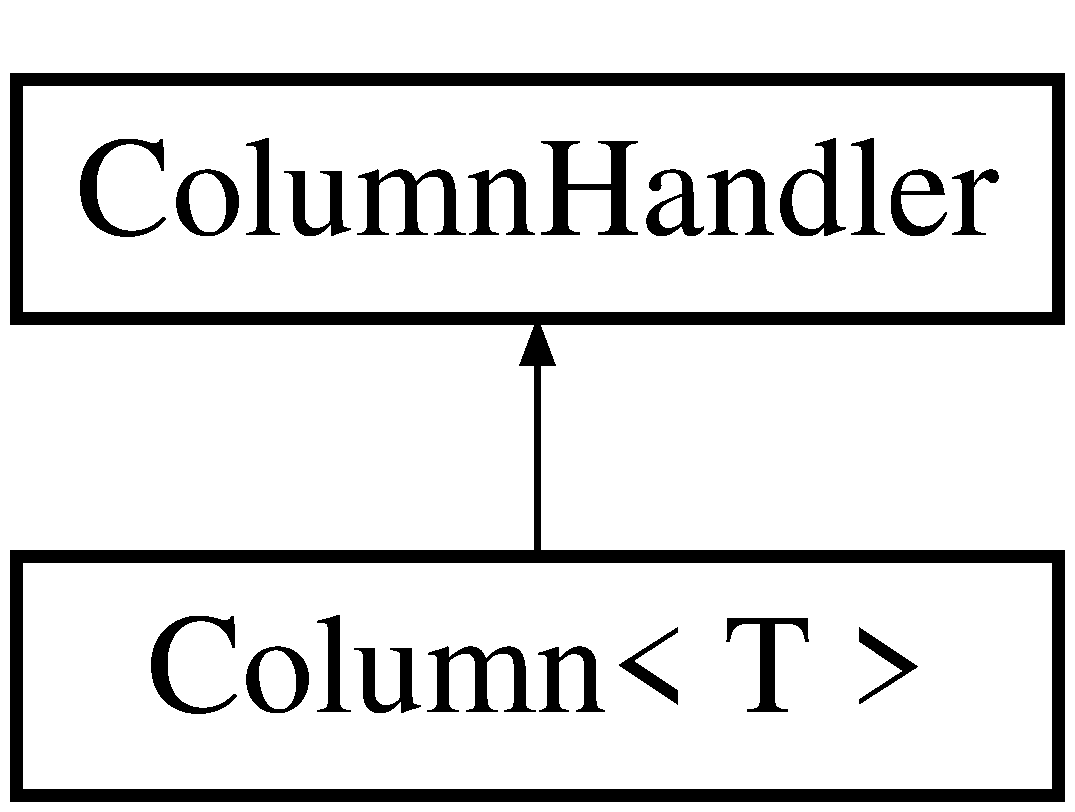
\includegraphics[height=2.000000cm]{class_column}
\end{center}
\end{figure}
\subsection*{Metody publiczne}
\begin{DoxyCompactItemize}
\item 
\mbox{\hyperlink{class_column_ac244a78d96a7a83cb2bf201a4b65cc60}{Column}} (std\+::string name\+Of\+Column, bool pk=false, bool fk=false, bool nullable=true, bool unique=false)
\begin{DoxyCompactList}\small\item\em Implementacje metod. \end{DoxyCompactList}\item 
\mbox{\hyperlink{class_column_a2563bd8f764ee4423fdb8426e5ff3d2d}{Column}} (std\+::string name\+Of\+Column, bool $\ast$flags)
\item 
\mbox{\Hypertarget{class_column_ac4dff6048d07de37b640caa291765c28}\label{class_column_ac4dff6048d07de37b640caa291765c28}} 
std\+::string \mbox{\hyperlink{class_column_ac4dff6048d07de37b640caa291765c28}{get\+Name}} ()
\begin{DoxyCompactList}\small\item\em Zwraca nazwe kolumny. \end{DoxyCompactList}\item 
\mbox{\Hypertarget{class_column_afb265d4dd087deed41448b68cfc7bb76}\label{class_column_afb265d4dd087deed41448b68cfc7bb76}} 
void \mbox{\hyperlink{class_column_afb265d4dd087deed41448b68cfc7bb76}{set\+Table\+Name}} (std\+::string table\+Name)
\begin{DoxyCompactList}\small\item\em Ustala nazwe tabeli obejmujacej (przyjmuje nazwe tabeli) \end{DoxyCompactList}\item 
\mbox{\Hypertarget{class_column_ae43964d7b88d4c9e7e357b285edc5ed5}\label{class_column_ae43964d7b88d4c9e7e357b285edc5ed5}} 
std\+::string \mbox{\hyperlink{class_column_ae43964d7b88d4c9e7e357b285edc5ed5}{get\+Table\+Name}} ()
\begin{DoxyCompactList}\small\item\em Zwraca nazwe tabeli obejmujacej. \end{DoxyCompactList}\item 
\mbox{\Hypertarget{class_column_a3e83b7a782fb92f5308122e522c8b8c4}\label{class_column_a3e83b7a782fb92f5308122e522c8b8c4}} 
void \mbox{\hyperlink{class_column_a3e83b7a782fb92f5308122e522c8b8c4}{add\+Value}} (const T \&value, int index=A\+R\+G\+\_\+\+N\+O\+T\+\_\+\+P\+R\+O\+V\+I\+D\+ED)
\begin{DoxyCompactList}\small\item\em Dodaj wartosc (przyjmuje wartosc, ktora ma zostac dodana oraz odpowiedni indeks) \end{DoxyCompactList}\item 
\mbox{\Hypertarget{class_column_ae31c40b1f30b13e1f05694792bf84fe3}\label{class_column_ae31c40b1f30b13e1f05694792bf84fe3}} 
void \mbox{\hyperlink{class_column_ae31c40b1f30b13e1f05694792bf84fe3}{add\+Null\+Value}} (unsigned int index=0)
\begin{DoxyCompactList}\small\item\em Dodaj puste pole (przyjmuje opdowiedni indeks) \end{DoxyCompactList}\item 
\mbox{\Hypertarget{class_column_ad451edfb49eca6136269ba885ba8f5f2}\label{class_column_ad451edfb49eca6136269ba885ba8f5f2}} 
void \mbox{\hyperlink{class_column_ad451edfb49eca6136269ba885ba8f5f2}{delete\+Value}} (unsigned int index)
\begin{DoxyCompactList}\small\item\em Usun wartosc (przyjmuje odpowiedni indeks) \end{DoxyCompactList}\item 
std\+::string \mbox{\hyperlink{class_column_a01f68d75e582070faf9b53e49a50c740}{stream\+Print}} (unsigned int index, bool file\+Print=false)
\item 
\mbox{\Hypertarget{class_column_a28f0dc54b6248de35dbe980ff33e3e35}\label{class_column_a28f0dc54b6248de35dbe980ff33e3e35}} 
unsigned int \mbox{\hyperlink{class_column_a28f0dc54b6248de35dbe980ff33e3e35}{get\+Column\+Size}} ()
\begin{DoxyCompactList}\small\item\em Zwraca rozmiar kolumny. \end{DoxyCompactList}\item 
\mbox{\Hypertarget{class_column_ae82ecb46ea5e8a5849dd437d03c5dd18}\label{class_column_ae82ecb46ea5e8a5849dd437d03c5dd18}} 
bool \mbox{\hyperlink{class_column_ae82ecb46ea5e8a5849dd437d03c5dd18}{is\+Nullable}} ()
\begin{DoxyCompactList}\small\item\em Zwraca czy kolumna moze miec puste pola. \end{DoxyCompactList}\item 
\mbox{\Hypertarget{class_column_a02a49330774bf62536d686757e84873b}\label{class_column_a02a49330774bf62536d686757e84873b}} 
bool \mbox{\hyperlink{class_column_a02a49330774bf62536d686757e84873b}{is\+Pk}} ()
\begin{DoxyCompactList}\small\item\em Zwraca czy kolumna jest kluczem glownym. \end{DoxyCompactList}\item 
\mbox{\Hypertarget{class_column_a8ec7fb1f80b67714e6b4963ed7237788}\label{class_column_a8ec7fb1f80b67714e6b4963ed7237788}} 
bool \mbox{\hyperlink{class_column_a8ec7fb1f80b67714e6b4963ed7237788}{is\+Fk}} ()
\begin{DoxyCompactList}\small\item\em Zwraca czy kolumna jest kluczem obcym. \end{DoxyCompactList}\item 
\mbox{\Hypertarget{class_column_a739b9804e0543ca88f215a7a42f9efe9}\label{class_column_a739b9804e0543ca88f215a7a42f9efe9}} 
bool \mbox{\hyperlink{class_column_a739b9804e0543ca88f215a7a42f9efe9}{is\+Unique}} ()
\begin{DoxyCompactList}\small\item\em Zwraca czy pola kolumny musza byc unikalne. \end{DoxyCompactList}\item 
\mbox{\Hypertarget{class_column_a676736d57fd4a0b6ffc35f20ab65cdcf}\label{class_column_a676736d57fd4a0b6ffc35f20ab65cdcf}} 
Column\+Type \mbox{\hyperlink{class_column_a676736d57fd4a0b6ffc35f20ab65cdcf}{what\+Type}} ()
\begin{DoxyCompactList}\small\item\em Zwraca typ kolumny w postaci odpowiedniego znaku. \end{DoxyCompactList}\end{DoxyCompactItemize}


\subsection{Opis szczegółowy}
\subsubsection*{template$<$typename T$>$\newline
class Column$<$ T $>$}

Klasa pochodna (glowna) Implementuje podstawowe operacje na kolumnie i jej polach 

Definicja w linii 36 pliku column.\+hpp.



\subsection{Dokumentacja konstruktora i destruktora}
\mbox{\Hypertarget{class_column_ac244a78d96a7a83cb2bf201a4b65cc60}\label{class_column_ac244a78d96a7a83cb2bf201a4b65cc60}} 
\index{Column@{Column}!Column@{Column}}
\index{Column@{Column}!Column@{Column}}
\subsubsection{\texorpdfstring{Column()}{Column()}\hspace{0.1cm}{\footnotesize\ttfamily [1/2]}}
{\footnotesize\ttfamily template$<$typename T $>$ \\
\mbox{\hyperlink{class_column}{Column}}$<$ T $>$\+::\mbox{\hyperlink{class_column}{Column}} (\begin{DoxyParamCaption}\item[{std\+::string}]{name\+Of\+Column,  }\item[{bool}]{pk = {\ttfamily false},  }\item[{bool}]{fk = {\ttfamily false},  }\item[{bool}]{nullable = {\ttfamily true},  }\item[{bool}]{unique = {\ttfamily false} }\end{DoxyParamCaption})}



Implementacje metod. 

Konstruktor kolumny inicjalizujacy jej parametry (przyjmuje nazwe nowej kolumny oraz opcjonalne odpowiednie parametry) 

Definicja w linii 8 pliku column.\+cpp.

\mbox{\Hypertarget{class_column_a2563bd8f764ee4423fdb8426e5ff3d2d}\label{class_column_a2563bd8f764ee4423fdb8426e5ff3d2d}} 
\index{Column@{Column}!Column@{Column}}
\index{Column@{Column}!Column@{Column}}
\subsubsection{\texorpdfstring{Column()}{Column()}\hspace{0.1cm}{\footnotesize\ttfamily [2/2]}}
{\footnotesize\ttfamily template$<$typename T $>$ \\
\mbox{\hyperlink{class_column}{Column}}$<$ T $>$\+::\mbox{\hyperlink{class_column}{Column}} (\begin{DoxyParamCaption}\item[{std\+::string}]{name\+Of\+Column,  }\item[{bool $\ast$}]{flags }\end{DoxyParamCaption})}

Opcjonalny konstruktor kolumny inicjalizujacy jej parametry (przyjmuje nazwe nowej kolumny oraz opcjonalne odpowiednie parametry) 

Definicja w linii 31 pliku column.\+cpp.



\subsection{Dokumentacja funkcji składowych}
\mbox{\Hypertarget{class_column_a01f68d75e582070faf9b53e49a50c740}\label{class_column_a01f68d75e582070faf9b53e49a50c740}} 
\index{Column@{Column}!stream\+Print@{stream\+Print}}
\index{stream\+Print@{stream\+Print}!Column@{Column}}
\subsubsection{\texorpdfstring{stream\+Print()}{streamPrint()}}
{\footnotesize\ttfamily template$<$typename T $>$ \\
std\+::string \mbox{\hyperlink{class_column}{Column}}$<$ T $>$\+::stream\+Print (\begin{DoxyParamCaption}\item[{unsigned int}]{index,  }\item[{bool}]{file\+Print = {\ttfamily false} }\end{DoxyParamCaption})\hspace{0.3cm}{\ttfamily [virtual]}}

Zwraca wartosc (przyjmuje odpowiedni indeks oraz flage okreslajaca typ zwracania wartosci null do plikow) 

Implementuje \mbox{\hyperlink{class_column_handler}{Column\+Handler}}.



Definicja w linii 141 pliku column.\+cpp.



Dokumentacja dla tej klasy została wygenerowana z plików\+:\begin{DoxyCompactItemize}
\item 
F\+:/\+Pobieranie/\+No\+S\+Q\+L-\/\+Database-\/master/src/column.\+hpp\item 
F\+:/\+Pobieranie/\+No\+S\+Q\+L-\/\+Database-\/master/src/column.\+cpp\end{DoxyCompactItemize}

\hypertarget{class_column_handler}{}\section{Dokumentacja klasy Column\+Handler}
\label{class_column_handler}\index{Column\+Handler@{Column\+Handler}}


{\ttfamily \#include $<$column.\+hpp$>$}

Diagram dziedziczenia dla Column\+Handler\begin{figure}[H]
\begin{center}
\leavevmode
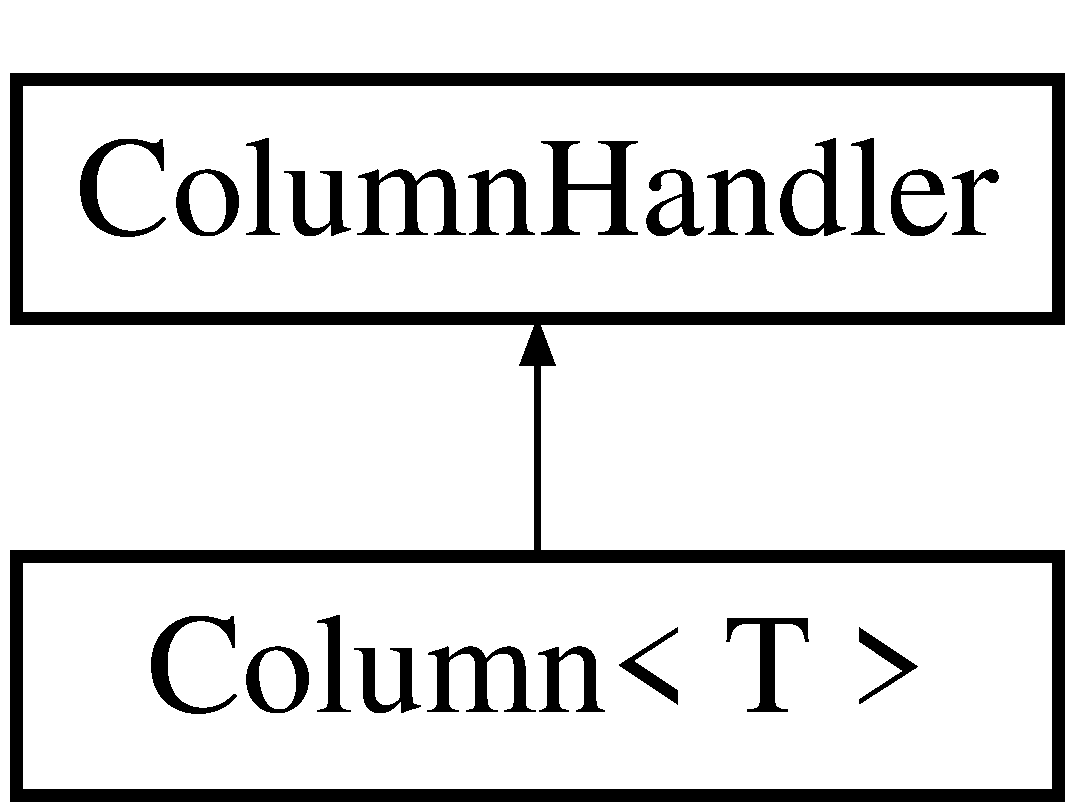
\includegraphics[height=2.000000cm]{class_column_handler}
\end{center}
\end{figure}
\subsection*{Metody publiczne}
\begin{DoxyCompactItemize}
\item 
\mbox{\Hypertarget{class_column_handler_a020bbf00c5b3ece65cb6122b1f17c749}\label{class_column_handler_a020bbf00c5b3ece65cb6122b1f17c749}} 
virtual std\+::string {\bfseries get\+Name} ()=0
\item 
\mbox{\Hypertarget{class_column_handler_a1b9efa4e5fcc8b788109772e59173a2a}\label{class_column_handler_a1b9efa4e5fcc8b788109772e59173a2a}} 
virtual void {\bfseries set\+Table\+Name} (std\+::string table\+Name)=0
\item 
\mbox{\Hypertarget{class_column_handler_a8dcfcbed92a3e1ed4d91ff88e5fcae6d}\label{class_column_handler_a8dcfcbed92a3e1ed4d91ff88e5fcae6d}} 
virtual std\+::string {\bfseries get\+Table\+Name} ()=0
\item 
\mbox{\Hypertarget{class_column_handler_a3d2b864155ffb3daeba5337654a42a94}\label{class_column_handler_a3d2b864155ffb3daeba5337654a42a94}} 
virtual void {\bfseries add\+Null\+Value} (unsigned int index=0)=0
\item 
\mbox{\Hypertarget{class_column_handler_aefd69e41261e8c0aa953c9f915762b80}\label{class_column_handler_aefd69e41261e8c0aa953c9f915762b80}} 
virtual void {\bfseries delete\+Value} (unsigned int index)=0
\item 
\mbox{\Hypertarget{class_column_handler_a184549518f6c45829b4b413d3b07055f}\label{class_column_handler_a184549518f6c45829b4b413d3b07055f}} 
virtual unsigned int {\bfseries get\+Column\+Size} ()=0
\item 
\mbox{\Hypertarget{class_column_handler_ab79c65f0e167f6c640f7d4daf92e9593}\label{class_column_handler_ab79c65f0e167f6c640f7d4daf92e9593}} 
virtual std\+::string {\bfseries stream\+Print} (unsigned int index, bool file\+Print=false)=0
\item 
\mbox{\Hypertarget{class_column_handler_a06482951220e9871cd7d51fcfd1d3729}\label{class_column_handler_a06482951220e9871cd7d51fcfd1d3729}} 
virtual bool {\bfseries is\+Nullable} ()=0
\item 
\mbox{\Hypertarget{class_column_handler_af296a21afca765c83e508038ba4bf070}\label{class_column_handler_af296a21afca765c83e508038ba4bf070}} 
virtual bool {\bfseries is\+Pk} ()=0
\item 
\mbox{\Hypertarget{class_column_handler_a22e64016cb2e0b35094d192fbab0d416}\label{class_column_handler_a22e64016cb2e0b35094d192fbab0d416}} 
virtual bool {\bfseries is\+Fk} ()=0
\item 
\mbox{\Hypertarget{class_column_handler_a375114cf104e5bd8147d66f30613ed6c}\label{class_column_handler_a375114cf104e5bd8147d66f30613ed6c}} 
virtual bool {\bfseries is\+Unique} ()=0
\item 
\mbox{\Hypertarget{class_column_handler_a353fdaaa60e433b2dacb87144ad7f0dd}\label{class_column_handler_a353fdaaa60e433b2dacb87144ad7f0dd}} 
virtual Column\+Type {\bfseries what\+Type} ()=0
\end{DoxyCompactItemize}


\subsection{Opis szczegółowy}
Klasa bazowa (dodatkowa) Jest zaimplementowana w celu ulatwienia przechowywania kolumn w tabelach (kolumny przechowywane sa w kontenerze Vector, ktory nie przechowuje szablonow klas) 

Definicja w linii 16 pliku column.\+hpp.



Dokumentacja dla tej klasy została wygenerowana z pliku\+:\begin{DoxyCompactItemize}
\item 
F\+:/\+Pobieranie/\+No\+S\+Q\+L-\/\+Database-\/master/src/column.\+hpp\end{DoxyCompactItemize}

\hypertarget{class_database}{}\section{Dokumentacja klasy Database}
\label{class_database}\index{Database@{Database}}


Klasa calej bazy danych zawierajacej tabele.  




{\ttfamily \#include $<$database.\+hpp$>$}

\subsection*{Metody publiczne}
\begin{DoxyCompactItemize}
\item 
\mbox{\hyperlink{class_database_aab14cbf95cbe114d24a2884e9417a102}{Database}} (std\+::string name\+Of\+Database, std\+::string database\+Filename)
\begin{DoxyCompactList}\small\item\em Implementacje metod. \end{DoxyCompactList}\item 
\mbox{\Hypertarget{class_database_a87aa575818688a5e589899bd3fa97ada}\label{class_database_a87aa575818688a5e589899bd3fa97ada}} 
std\+::string \mbox{\hyperlink{class_database_a87aa575818688a5e589899bd3fa97ada}{get\+Name}} ()
\begin{DoxyCompactList}\small\item\em Zwraca nazwe bazy danych. \end{DoxyCompactList}\item 
\mbox{\Hypertarget{class_database_ae96b8e91b8119131e101555cbddb4308}\label{class_database_ae96b8e91b8119131e101555cbddb4308}} 
void \mbox{\hyperlink{class_database_ae96b8e91b8119131e101555cbddb4308}{set\+Name}} (std\+::string database\+Name)
\begin{DoxyCompactList}\small\item\em Ustawia nazwe bazy danych. \end{DoxyCompactList}\item 
\mbox{\Hypertarget{class_database_ac5c3a78c9bdcd6462cd6e9e0f77d5fa7}\label{class_database_ac5c3a78c9bdcd6462cd6e9e0f77d5fa7}} 
unsigned int \mbox{\hyperlink{class_database_ac5c3a78c9bdcd6462cd6e9e0f77d5fa7}{get\+Database\+Size}} ()
\begin{DoxyCompactList}\small\item\em Zwraca ilosc tabel w bazie danych. \end{DoxyCompactList}\item 
\mbox{\Hypertarget{class_database_a289b0374a783122e3fc62017b1a4f2d2}\label{class_database_a289b0374a783122e3fc62017b1a4f2d2}} 
void \mbox{\hyperlink{class_database_a289b0374a783122e3fc62017b1a4f2d2}{clear\+Database}} ()
\begin{DoxyCompactList}\small\item\em Wyczysc cala baze danych. \end{DoxyCompactList}\item 
bool \mbox{\hyperlink{class_database_ac0427d3cb0807610d5b5d2c2e910d95c}{attach\+Table\+To\+Database}} (\mbox{\hyperlink{class_table}{Table}} $\ast$table)
\item 
\mbox{\Hypertarget{class_database_affa35fc28233e8c1bcce587cd0bfcf1a}\label{class_database_affa35fc28233e8c1bcce587cd0bfcf1a}} 
void \mbox{\hyperlink{class_database_affa35fc28233e8c1bcce587cd0bfcf1a}{detach\+Table\+From\+Database}} (unsigned int index)
\begin{DoxyCompactList}\small\item\em Odlacz tabele z bazy danych. \end{DoxyCompactList}\item 
\mbox{\Hypertarget{class_database_a1b96ea42ef05966cbefddc0f58f62309}\label{class_database_a1b96ea42ef05966cbefddc0f58f62309}} 
void \mbox{\hyperlink{class_database_a1b96ea42ef05966cbefddc0f58f62309}{print\+Database}} ()
\begin{DoxyCompactList}\small\item\em Wyswietla cala baze danych. \end{DoxyCompactList}\item 
\mbox{\Hypertarget{class_database_a5c807d796ad3dd3b1bec1022f6716384}\label{class_database_a5c807d796ad3dd3b1bec1022f6716384}} 
void \mbox{\hyperlink{class_database_a5c807d796ad3dd3b1bec1022f6716384}{set\+Pk}} (\mbox{\hyperlink{class_column_handler}{Column\+Handler}} $\ast$pk\+Column)
\begin{DoxyCompactList}\small\item\em Dodaje polaczenie klucza glownego (przyjmuje glowna kolumne) \end{DoxyCompactList}\item 
\mbox{\Hypertarget{class_database_a2829a5d8fae11a7321a77bba69e0af94}\label{class_database_a2829a5d8fae11a7321a77bba69e0af94}} 
void \mbox{\hyperlink{class_database_a2829a5d8fae11a7321a77bba69e0af94}{set\+Fk}} (\mbox{\hyperlink{class_column_handler}{Column\+Handler}} $\ast$fk\+Column)
\begin{DoxyCompactList}\small\item\em Dodaje polaczenie klucza obcego (przyjmuje obca kolumne) \end{DoxyCompactList}\item 
\mbox{\Hypertarget{class_database_ac153fb7c7534f137a359a98095f21043}\label{class_database_ac153fb7c7534f137a359a98095f21043}} 
void \mbox{\hyperlink{class_database_ac153fb7c7534f137a359a98095f21043}{delete\+Pk}} (\mbox{\hyperlink{class_column_handler}{Column\+Handler}} $\ast$pk\+Column)
\begin{DoxyCompactList}\small\item\em Usuwa polaczenie klucza glownego (przyjmuje glowna kolumne) \end{DoxyCompactList}\item 
\mbox{\Hypertarget{class_database_aa14d473d6896af6f530b1cd2875a22ca}\label{class_database_aa14d473d6896af6f530b1cd2875a22ca}} 
void \mbox{\hyperlink{class_database_aa14d473d6896af6f530b1cd2875a22ca}{delete\+Fk}} (\mbox{\hyperlink{class_column_handler}{Column\+Handler}} $\ast$fk\+Column)
\begin{DoxyCompactList}\small\item\em Usuwa polaczenie klucza obcego (przyjmuje obca kolumne) \end{DoxyCompactList}\item 
\mbox{\Hypertarget{class_database_a177cf4f47f1621c9fdc6ef02c79f15d5}\label{class_database_a177cf4f47f1621c9fdc6ef02c79f15d5}} 
std\+::string \mbox{\hyperlink{class_database_a177cf4f47f1621c9fdc6ef02c79f15d5}{get\+Keys\+String}} ()
\begin{DoxyCompactList}\small\item\em Zwraca wszystkie polaczenia miedzy tabelami. \end{DoxyCompactList}\item 
\mbox{\hyperlink{class_table}{Table}} $\ast$ \mbox{\hyperlink{class_database_a3e26371207ec61140b3853e606577d57}{get\+Table}} (std\+::string name\+Of\+Table)
\item 
\mbox{\Hypertarget{class_database_aeddeeeb63684a663c7f6f46e406ae84e}\label{class_database_aeddeeeb63684a663c7f6f46e406ae84e}} 
\mbox{\hyperlink{class_table}{Table}} $\ast$ {\bfseries get\+Table} (unsigned int index)
\item 
bool \mbox{\hyperlink{class_database_a8e8b77a7b47bc487e32f81bc34524e10}{contains\+Table}} (std\+::string name\+Of\+Table)
\item 
\mbox{\Hypertarget{class_database_afefb0dc79154a0ec6d6ad80df11c6959}\label{class_database_afefb0dc79154a0ec6d6ad80df11c6959}} 
bool \mbox{\hyperlink{class_database_afefb0dc79154a0ec6d6ad80df11c6959}{empty}} ()
\begin{DoxyCompactList}\small\item\em Sprawdza czy baza danych jest pusta (Zwraca prawde lub falsz) \end{DoxyCompactList}\item 
\mbox{\Hypertarget{class_database_a1d055600cbd151eef4a2dd7989a2ab80}\label{class_database_a1d055600cbd151eef4a2dd7989a2ab80}} 
bool \mbox{\hyperlink{class_database_a1d055600cbd151eef4a2dd7989a2ab80}{keys\+Empty}} ()
\begin{DoxyCompactList}\small\item\em Sprawdza czy w bazie danych znajduja sie jakies polaczenia. \end{DoxyCompactList}\item 
\mbox{\Hypertarget{class_database_a68c01178477790e27ae69cced3a0b437}\label{class_database_a68c01178477790e27ae69cced3a0b437}} 
void \mbox{\hyperlink{class_database_a68c01178477790e27ae69cced3a0b437}{save\+Database}} ()
\begin{DoxyCompactList}\small\item\em Zapisuje baze danych do pliku lokalnego. \end{DoxyCompactList}\item 
bool \mbox{\hyperlink{class_database_a8ce06beb2fbd98398e0309e55a093508}{load\+Database}} (std\+::string \&time)
\end{DoxyCompactItemize}


\subsection{Opis szczegółowy}
Klasa calej bazy danych zawierajacej tabele. 

Definicja w linii 12 pliku database.\+hpp.



\subsection{Dokumentacja konstruktora i destruktora}
\mbox{\Hypertarget{class_database_aab14cbf95cbe114d24a2884e9417a102}\label{class_database_aab14cbf95cbe114d24a2884e9417a102}} 
\index{Database@{Database}!Database@{Database}}
\index{Database@{Database}!Database@{Database}}
\subsubsection{\texorpdfstring{Database()}{Database()}}
{\footnotesize\ttfamily Database\+::\+Database (\begin{DoxyParamCaption}\item[{std\+::string}]{name\+Of\+Database,  }\item[{std\+::string}]{database\+Filename }\end{DoxyParamCaption})}



Implementacje metod. 

Konstruktor bazy danych (przyjmuje nazwe bazy danych, nazwe pliku lokalnego i wskaznik sprawdzajacy czy poprawnie otwarto plik) 

Definicja w linii 7 pliku database.\+cpp.



\subsection{Dokumentacja funkcji składowych}
\mbox{\Hypertarget{class_database_ac0427d3cb0807610d5b5d2c2e910d95c}\label{class_database_ac0427d3cb0807610d5b5d2c2e910d95c}} 
\index{Database@{Database}!attach\+Table\+To\+Database@{attach\+Table\+To\+Database}}
\index{attach\+Table\+To\+Database@{attach\+Table\+To\+Database}!Database@{Database}}
\subsubsection{\texorpdfstring{attach\+Table\+To\+Database()}{attachTableToDatabase()}}
{\footnotesize\ttfamily bool Database\+::attach\+Table\+To\+Database (\begin{DoxyParamCaption}\item[{\mbox{\hyperlink{class_table}{Table}} $\ast$}]{table }\end{DoxyParamCaption})}

Podlacz tabele do bazy bazy danych (zwraca flage, ktora mowi o tym czy udalo sie dolaczyc tabele) 

Definicja w linii 35 pliku database.\+cpp.

\mbox{\Hypertarget{class_database_a8e8b77a7b47bc487e32f81bc34524e10}\label{class_database_a8e8b77a7b47bc487e32f81bc34524e10}} 
\index{Database@{Database}!contains\+Table@{contains\+Table}}
\index{contains\+Table@{contains\+Table}!Database@{Database}}
\subsubsection{\texorpdfstring{contains\+Table()}{containsTable()}}
{\footnotesize\ttfamily bool Database\+::contains\+Table (\begin{DoxyParamCaption}\item[{std\+::string}]{name\+Of\+Table }\end{DoxyParamCaption})}

Sprawdza czy tabela znajduje sie w bazie danych (przyjmuje nazwe tabeli, zwraca prawde lub falsz) 

Definicja w linii 157 pliku database.\+cpp.

\mbox{\Hypertarget{class_database_a3e26371207ec61140b3853e606577d57}\label{class_database_a3e26371207ec61140b3853e606577d57}} 
\index{Database@{Database}!get\+Table@{get\+Table}}
\index{get\+Table@{get\+Table}!Database@{Database}}
\subsubsection{\texorpdfstring{get\+Table()}{getTable()}}
{\footnotesize\ttfamily \mbox{\hyperlink{class_table}{Table}} $\ast$ Database\+::get\+Table (\begin{DoxyParamCaption}\item[{std\+::string}]{name\+Of\+Table }\end{DoxyParamCaption})}

Zwraca wskaznik na dana tabele (przyjmuje nazwe tabeli lub odpowiedni indeks) 

Definicja w linii 141 pliku database.\+cpp.

\mbox{\Hypertarget{class_database_a8ce06beb2fbd98398e0309e55a093508}\label{class_database_a8ce06beb2fbd98398e0309e55a093508}} 
\index{Database@{Database}!load\+Database@{load\+Database}}
\index{load\+Database@{load\+Database}!Database@{Database}}
\subsubsection{\texorpdfstring{load\+Database()}{loadDatabase()}}
{\footnotesize\ttfamily bool Database\+::load\+Database (\begin{DoxyParamCaption}\item[{std\+::string \&}]{time }\end{DoxyParamCaption})}

Odczytuje baze danych z pliku lokalnego (zwraca flage czy powiodlo sie odczytywanie pliku) 

Definicja w linii 246 pliku database.\+cpp.



Dokumentacja dla tej klasy została wygenerowana z plików\+:\begin{DoxyCompactItemize}
\item 
F\+:/\+Pobieranie/\+No\+S\+Q\+L-\/\+Database-\/master/src/database.\+hpp\item 
F\+:/\+Pobieranie/\+No\+S\+Q\+L-\/\+Database-\/master/src/database.\+cpp\end{DoxyCompactItemize}

\hypertarget{class_display}{}\section{Dokumentacja klasy Display}
\label{class_display}\index{Display@{Display}}


Klasa Wyjscia odpowiadajaca za komunikacje z uzytkownikiem.  




{\ttfamily \#include $<$display.\+hpp$>$}

\subsection*{Metody publiczne}
\begin{DoxyCompactItemize}
\item 
\mbox{\Hypertarget{class_display_a29169f26fa9668f8a370d1c26bc7d5ba}\label{class_display_a29169f26fa9668f8a370d1c26bc7d5ba}} 
void \mbox{\hyperlink{class_display_a29169f26fa9668f8a370d1c26bc7d5ba}{connect\+Database}} (\mbox{\hyperlink{class_database}{Database}} $\ast$database)
\begin{DoxyCompactList}\small\item\em Laczy baze danych. \end{DoxyCompactList}\item 
\mbox{\Hypertarget{class_display_a42cdd77de47fd4ebd5a99cfbe1fdba3b}\label{class_display_a42cdd77de47fd4ebd5a99cfbe1fdba3b}} 
void \mbox{\hyperlink{class_display_a42cdd77de47fd4ebd5a99cfbe1fdba3b}{destroy\+Display}} ()
\begin{DoxyCompactList}\small\item\em Wywoluje destruktor obiektu -\/ konczy prace klasy wyjscia. \end{DoxyCompactList}\item 
\mbox{\Hypertarget{class_display_a7a1dce8e6c3149170ecbffc983d2a859}\label{class_display_a7a1dce8e6c3149170ecbffc983d2a859}} 
std\+::string \mbox{\hyperlink{class_display_a7a1dce8e6c3149170ecbffc983d2a859}{get\+Database\+Name}} ()
\begin{DoxyCompactList}\small\item\em Metoda pobierajaca nazwe bazy danych. \end{DoxyCompactList}\item 
\mbox{\Hypertarget{class_display_ac4e3345a1de41423b538343d3c4f77d2}\label{class_display_ac4e3345a1de41423b538343d3c4f77d2}} 
void \mbox{\hyperlink{class_display_ac4e3345a1de41423b538343d3c4f77d2}{start\+Main\+Menu}} ()
\begin{DoxyCompactList}\small\item\em Uruchamia menu glowne. \end{DoxyCompactList}\end{DoxyCompactItemize}
\subsection*{Statyczne metody publiczne}
\begin{DoxyCompactItemize}
\item 
\mbox{\Hypertarget{class_display_a38528a0104dcd6822e2b0148bbcd113c}\label{class_display_a38528a0104dcd6822e2b0148bbcd113c}} 
static \mbox{\hyperlink{class_display}{Display}} $\ast$ \mbox{\hyperlink{class_display_a38528a0104dcd6822e2b0148bbcd113c}{init\+Display}} ()
\begin{DoxyCompactList}\small\item\em Zainicjuj klase wyjscia (Zwraca pojedynczy obiekt) \end{DoxyCompactList}\end{DoxyCompactItemize}


\subsection{Opis szczegółowy}
Klasa Wyjscia odpowiadajaca za komunikacje z uzytkownikiem. 

Definicja w linii 8 pliku display.\+hpp.



Dokumentacja dla tej klasy została wygenerowana z plików\+:\begin{DoxyCompactItemize}
\item 
F\+:/\+Pobieranie/\+No\+S\+Q\+L-\/\+Database-\/master/src/display.\+hpp\item 
F\+:/\+Pobieranie/\+No\+S\+Q\+L-\/\+Database-\/master/src/display.\+cpp\end{DoxyCompactItemize}

\hypertarget{class_menu}{}\section{Dokumentacja klasy Menu}
\label{class_menu}\index{Menu@{Menu}}
\subsection*{Statyczne metody publiczne}
\begin{DoxyCompactItemize}
\item 
static void \mbox{\hyperlink{class_menu_ad413f4b72438f65886bc5f5e370ad426}{print\+Menu\+Choices}} (W\+I\+N\+D\+OW $\ast$window, Choices\+::choices\+\_\+t which\+Menu, unsigned int highlight, std\+::string database\+Name)
\begin{DoxyCompactList}\small\item\em Implementacja metod. \end{DoxyCompactList}\item 
static void \mbox{\hyperlink{class_menu_a5faa9cd8e2be7ef81916032c64a1d460}{print\+Menu\+Choices}} (W\+I\+N\+D\+OW $\ast$window, const std\+::string $\ast$menu\+Choices, unsigned int size, std\+::string window\+Name, std\+::string database\+Name, unsigned int highlight)
\item 
static int \mbox{\hyperlink{class_menu_a452bfc7ce14d367bdf38cee636f09b0c}{draw\+Menu}} (W\+I\+N\+D\+OW $\ast$window, Choices\+::choices\+\_\+t which\+Menu, std\+::string database\+Name)
\item 
static int \mbox{\hyperlink{class_menu_a8c2a73e33c0cbf1a8b09b2c4831ea2b8}{draw\+Menu}} (W\+I\+N\+D\+OW $\ast$window, const std\+::string menu\+Choices\mbox{[}$\,$\mbox{]}, unsigned int size, std\+::string window\+Name, std\+::string database\+Name)
\item 
static void \mbox{\hyperlink{class_menu_aea098dfc2a133fae9e4b1c3c31bdc448}{print\+Horizontal\+Menu\+Choices}} (W\+I\+N\+D\+OW $\ast$window, const std\+::string $\ast$menu\+Choices, unsigned int size, unsigned int shift, unsigned int highlight)
\item 
static int \mbox{\hyperlink{class_menu_a22e5c26ac2b73a702749a0229ad4fcba}{draw\+Horizontal\+Menu}} (W\+I\+N\+D\+OW $\ast$window, const std\+::string $\ast$menu\+Choices, unsigned int size, unsigned int shift)
\item 
static void \mbox{\hyperlink{class_menu_afcf3606c830a65335e61b1d0bd4e432a}{print\+Menu\+Selectable}} (W\+I\+N\+D\+OW $\ast$window, const std\+::string $\ast$menu\+Choices, unsigned int size, unsigned int shift, unsigned int highlight, bool $\ast$selected)
\item 
static bool $\ast$ \mbox{\hyperlink{class_menu_adf2ca061cdf65bd87500c74c1f1c2584}{draw\+Menu\+Selectable}} (W\+I\+N\+D\+OW $\ast$window, const std\+::string $\ast$menu\+Choices, unsigned int size, unsigned int shift)
\end{DoxyCompactItemize}
\subsection*{Statyczne atrybuty publiczne}
\begin{DoxyCompactItemize}
\item 
\mbox{\Hypertarget{class_menu_a2b3a53b8e554105fd9cf078604f1d455}\label{class_menu_a2b3a53b8e554105fd9cf078604f1d455}} 
static const int \mbox{\hyperlink{class_menu_a2b3a53b8e554105fd9cf078604f1d455}{main\+Menu\+Size\+Factor}} = 10
\begin{DoxyCompactList}\small\item\em Atrybuty okien. \end{DoxyCompactList}\end{DoxyCompactItemize}


\subsection{Opis szczegółowy}


Definicja w linii 46 pliku menu.\+hpp.



\subsection{Dokumentacja funkcji składowych}
\mbox{\Hypertarget{class_menu_a22e5c26ac2b73a702749a0229ad4fcba}\label{class_menu_a22e5c26ac2b73a702749a0229ad4fcba}} 
\index{Menu@{Menu}!draw\+Horizontal\+Menu@{draw\+Horizontal\+Menu}}
\index{draw\+Horizontal\+Menu@{draw\+Horizontal\+Menu}!Menu@{Menu}}
\subsubsection{\texorpdfstring{draw\+Horizontal\+Menu()}{drawHorizontalMenu()}}
{\footnotesize\ttfamily int Menu\+::draw\+Horizontal\+Menu (\begin{DoxyParamCaption}\item[{W\+I\+N\+D\+OW $\ast$}]{window,  }\item[{const std\+::string $\ast$}]{menu\+Choices,  }\item[{unsigned int}]{size,  }\item[{unsigned int}]{shift }\end{DoxyParamCaption})\hspace{0.3cm}{\ttfamily [static]}}

Rysuje poziome menu (Przyjmuje odpowiednie okno, pozycje menu, rozmiar tabeli oraz pionowe polozenie) 

Definicja w linii 167 pliku menu.\+cpp.

\mbox{\Hypertarget{class_menu_a452bfc7ce14d367bdf38cee636f09b0c}\label{class_menu_a452bfc7ce14d367bdf38cee636f09b0c}} 
\index{Menu@{Menu}!draw\+Menu@{draw\+Menu}}
\index{draw\+Menu@{draw\+Menu}!Menu@{Menu}}
\subsubsection{\texorpdfstring{draw\+Menu()}{drawMenu()}\hspace{0.1cm}{\footnotesize\ttfamily [1/2]}}
{\footnotesize\ttfamily int Menu\+::draw\+Menu (\begin{DoxyParamCaption}\item[{W\+I\+N\+D\+OW $\ast$}]{window,  }\item[{Choices\+::choices\+\_\+t}]{which\+Menu,  }\item[{std\+::string}]{database\+Name }\end{DoxyParamCaption})\hspace{0.3cm}{\ttfamily [static]}}

Rysuje menu (Przyjmuje okno, argument, ktore okno ma rysowac oraz nazwe bazy danych, zwraca liczbe calkowita oznaczajaca wybor) 

Definicja w linii 53 pliku menu.\+cpp.

\mbox{\Hypertarget{class_menu_a8c2a73e33c0cbf1a8b09b2c4831ea2b8}\label{class_menu_a8c2a73e33c0cbf1a8b09b2c4831ea2b8}} 
\index{Menu@{Menu}!draw\+Menu@{draw\+Menu}}
\index{draw\+Menu@{draw\+Menu}!Menu@{Menu}}
\subsubsection{\texorpdfstring{draw\+Menu()}{drawMenu()}\hspace{0.1cm}{\footnotesize\ttfamily [2/2]}}
{\footnotesize\ttfamily int Menu\+::draw\+Menu (\begin{DoxyParamCaption}\item[{W\+I\+N\+D\+OW $\ast$}]{window,  }\item[{const std\+::string}]{menu\+Choices\mbox{[}$\,$\mbox{]},  }\item[{unsigned int}]{size,  }\item[{std\+::string}]{window\+Name,  }\item[{std\+::string}]{database\+Name }\end{DoxyParamCaption})\hspace{0.3cm}{\ttfamily [static]}}

Przeciazona wersja rysowania menu (Przyjmuje pozycje menu, rozmiar tabeli, nazwe okna oraz nazwe bazy danych) 

Definicja w linii 97 pliku menu.\+cpp.

\mbox{\Hypertarget{class_menu_adf2ca061cdf65bd87500c74c1f1c2584}\label{class_menu_adf2ca061cdf65bd87500c74c1f1c2584}} 
\index{Menu@{Menu}!draw\+Menu\+Selectable@{draw\+Menu\+Selectable}}
\index{draw\+Menu\+Selectable@{draw\+Menu\+Selectable}!Menu@{Menu}}
\subsubsection{\texorpdfstring{draw\+Menu\+Selectable()}{drawMenuSelectable()}}
{\footnotesize\ttfamily bool $\ast$ Menu\+::draw\+Menu\+Selectable (\begin{DoxyParamCaption}\item[{W\+I\+N\+D\+OW $\ast$}]{window,  }\item[{const std\+::string $\ast$}]{menu\+Choices,  }\item[{unsigned int}]{size,  }\item[{unsigned int}]{shift }\end{DoxyParamCaption})\hspace{0.3cm}{\ttfamily [static]}}

Rysuje menu z zaznaczeniem (Przyjmuje pozycje menu, rozmiar tabeli, pionowe polozenie, zwraca tablice flag zaznaczenia) 

Definicja w linii 237 pliku menu.\+cpp.

\mbox{\Hypertarget{class_menu_aea098dfc2a133fae9e4b1c3c31bdc448}\label{class_menu_aea098dfc2a133fae9e4b1c3c31bdc448}} 
\index{Menu@{Menu}!print\+Horizontal\+Menu\+Choices@{print\+Horizontal\+Menu\+Choices}}
\index{print\+Horizontal\+Menu\+Choices@{print\+Horizontal\+Menu\+Choices}!Menu@{Menu}}
\subsubsection{\texorpdfstring{print\+Horizontal\+Menu\+Choices()}{printHorizontalMenuChoices()}}
{\footnotesize\ttfamily void Menu\+::print\+Horizontal\+Menu\+Choices (\begin{DoxyParamCaption}\item[{W\+I\+N\+D\+OW $\ast$}]{window,  }\item[{const std\+::string $\ast$}]{menu\+Choices,  }\item[{unsigned int}]{size,  }\item[{unsigned int}]{shift,  }\item[{unsigned int}]{highlight }\end{DoxyParamCaption})\hspace{0.3cm}{\ttfamily [static]}}

Wypisuje poziome menu (Przyjmuje odpowiednie okno pozycje menu, rozmiar tabeli, pionowe polozenie oraz odpowiednie podswietlenie) 

Definicja w linii 142 pliku menu.\+cpp.

\mbox{\Hypertarget{class_menu_ad413f4b72438f65886bc5f5e370ad426}\label{class_menu_ad413f4b72438f65886bc5f5e370ad426}} 
\index{Menu@{Menu}!print\+Menu\+Choices@{print\+Menu\+Choices}}
\index{print\+Menu\+Choices@{print\+Menu\+Choices}!Menu@{Menu}}
\subsubsection{\texorpdfstring{print\+Menu\+Choices()}{printMenuChoices()}\hspace{0.1cm}{\footnotesize\ttfamily [1/2]}}
{\footnotesize\ttfamily void Menu\+::print\+Menu\+Choices (\begin{DoxyParamCaption}\item[{W\+I\+N\+D\+OW $\ast$}]{window,  }\item[{Choices\+::choices\+\_\+t}]{which\+Menu,  }\item[{unsigned int}]{highlight,  }\item[{std\+::string}]{database\+Name }\end{DoxyParamCaption})\hspace{0.3cm}{\ttfamily [static]}}



Implementacja metod. 

Wypisuje menu (Przyjmuje okno, argument, ktore okno ma wypisac, odpowiednie podswietlenie oraz nazwe bazy danych) 

Definicja w linii 5 pliku menu.\+cpp.

\mbox{\Hypertarget{class_menu_a5faa9cd8e2be7ef81916032c64a1d460}\label{class_menu_a5faa9cd8e2be7ef81916032c64a1d460}} 
\index{Menu@{Menu}!print\+Menu\+Choices@{print\+Menu\+Choices}}
\index{print\+Menu\+Choices@{print\+Menu\+Choices}!Menu@{Menu}}
\subsubsection{\texorpdfstring{print\+Menu\+Choices()}{printMenuChoices()}\hspace{0.1cm}{\footnotesize\ttfamily [2/2]}}
{\footnotesize\ttfamily void Menu\+::print\+Menu\+Choices (\begin{DoxyParamCaption}\item[{W\+I\+N\+D\+OW $\ast$}]{window,  }\item[{const std\+::string $\ast$}]{menu\+Choices,  }\item[{unsigned int}]{size,  }\item[{std\+::string}]{window\+Name,  }\item[{std\+::string}]{database\+Name,  }\item[{unsigned int}]{highlight }\end{DoxyParamCaption})\hspace{0.3cm}{\ttfamily [static]}}

Przeciazona wersja rysowania menu (Przyjmuje okno, pozycje menu, rozmiar tabel, nazwe okna, nazwe bazy danych oraz odpowiednie podswietlenie) 

Definicja w linii 29 pliku menu.\+cpp.

\mbox{\Hypertarget{class_menu_afcf3606c830a65335e61b1d0bd4e432a}\label{class_menu_afcf3606c830a65335e61b1d0bd4e432a}} 
\index{Menu@{Menu}!print\+Menu\+Selectable@{print\+Menu\+Selectable}}
\index{print\+Menu\+Selectable@{print\+Menu\+Selectable}!Menu@{Menu}}
\subsubsection{\texorpdfstring{print\+Menu\+Selectable()}{printMenuSelectable()}}
{\footnotesize\ttfamily void Menu\+::print\+Menu\+Selectable (\begin{DoxyParamCaption}\item[{W\+I\+N\+D\+OW $\ast$}]{window,  }\item[{const std\+::string $\ast$}]{menu\+Choices,  }\item[{unsigned int}]{size,  }\item[{unsigned int}]{shift,  }\item[{unsigned int}]{highlight,  }\item[{bool $\ast$}]{selected }\end{DoxyParamCaption})\hspace{0.3cm}{\ttfamily [static]}}

Wypisuje menu z zaznaczeniem (Przyjmuje okno, pozycje menu, rozmiar tabeli, pionowe polozenie, odpowiednie podswietlenie i tablice flag zaznaczenia) 

Definicja w linii 207 pliku menu.\+cpp.



Dokumentacja dla tej klasy została wygenerowana z plików\+:\begin{DoxyCompactItemize}
\item 
F\+:/\+Pobieranie/\+No\+S\+Q\+L-\/\+Database-\/master/src/menu.\+hpp\item 
F\+:/\+Pobieranie/\+No\+S\+Q\+L-\/\+Database-\/master/src/menu.\+cpp\end{DoxyCompactItemize}

\hypertarget{class_operations}{}\section{Dokumentacja klasy Operations}
\label{class_operations}\index{Operations@{Operations}}


Klasa implementujaca poszczegolne operacje na bazie danych.  




{\ttfamily \#include $<$operations.\+hpp$>$}

\subsection*{Statyczne metody publiczne}
\begin{DoxyCompactItemize}
\item 
static void \mbox{\hyperlink{class_operations_a0d787c05e02fa042225975ffc31b84ad}{draw\+Database}} (\mbox{\hyperlink{class_database}{Database}} $\ast$database)
\begin{DoxyCompactList}\small\item\em Rysuje cala baze danych. \end{DoxyCompactList}\item 
\mbox{\Hypertarget{class_operations_a9db1b3adc8aeb0a297910b031065ca09}\label{class_operations_a9db1b3adc8aeb0a297910b031065ca09}} 
static bool \mbox{\hyperlink{class_operations_a9db1b3adc8aeb0a297910b031065ca09}{draw\+Database\+Keys}} (\mbox{\hyperlink{class_database}{Database}} $\ast$database)
\begin{DoxyCompactList}\small\item\em Wypisuje wszystkie klucze (Zwraca flage, ktora okresla powrot do menu) \end{DoxyCompactList}\item 
\mbox{\Hypertarget{class_operations_a08dcd1587e343a6ae8fb9499aa0d5e51}\label{class_operations_a08dcd1587e343a6ae8fb9499aa0d5e51}} 
static void \mbox{\hyperlink{class_operations_a08dcd1587e343a6ae8fb9499aa0d5e51}{draw\+Add\+Menu}} (\mbox{\hyperlink{class_database}{Database}} $\ast$database)
\begin{DoxyCompactList}\small\item\em Rysuje menu dodawania. \end{DoxyCompactList}\item 
\mbox{\Hypertarget{class_operations_aba6a02ac9ffff887460a1f7ea0423074}\label{class_operations_aba6a02ac9ffff887460a1f7ea0423074}} 
static bool \mbox{\hyperlink{class_operations_aba6a02ac9ffff887460a1f7ea0423074}{add\+Table}} (\mbox{\hyperlink{class_database}{Database}} $\ast$database)
\begin{DoxyCompactList}\small\item\em Dodaje tabele (Zwraca flage, ktora okresla powrot do menu) \end{DoxyCompactList}\item 
\mbox{\Hypertarget{class_operations_a20a8daf97c43a25ee11d4c208c14be3a}\label{class_operations_a20a8daf97c43a25ee11d4c208c14be3a}} 
static bool \mbox{\hyperlink{class_operations_a20a8daf97c43a25ee11d4c208c14be3a}{add\+Column}} (\mbox{\hyperlink{class_database}{Database}} $\ast$database)
\begin{DoxyCompactList}\small\item\em Dodaj kolumne (Zwraca flage, ktora okresla powrot do menu) \end{DoxyCompactList}\item 
\mbox{\Hypertarget{class_operations_afd7a5917e3bf9d5400938bdf8b739835}\label{class_operations_afd7a5917e3bf9d5400938bdf8b739835}} 
static bool \mbox{\hyperlink{class_operations_afd7a5917e3bf9d5400938bdf8b739835}{add\+Record}} (\mbox{\hyperlink{class_database}{Database}} $\ast$database)
\begin{DoxyCompactList}\small\item\em Dodaje rekord (Zwraca flage, ktora okresla powrot do menu) \end{DoxyCompactList}\item 
\mbox{\Hypertarget{class_operations_af80abbc0ef95dfe51598e17f090e5025}\label{class_operations_af80abbc0ef95dfe51598e17f090e5025}} 
static void \mbox{\hyperlink{class_operations_af80abbc0ef95dfe51598e17f090e5025}{draw\+Delete\+Menu}} (\mbox{\hyperlink{class_database}{Database}} $\ast$database)
\begin{DoxyCompactList}\small\item\em Rysuje menu usuwania. \end{DoxyCompactList}\item 
\mbox{\Hypertarget{class_operations_a0264d0eab5834bb2a7c4bd1a3123750b}\label{class_operations_a0264d0eab5834bb2a7c4bd1a3123750b}} 
static bool \mbox{\hyperlink{class_operations_a0264d0eab5834bb2a7c4bd1a3123750b}{delete\+Table}} (\mbox{\hyperlink{class_database}{Database}} $\ast$database)
\begin{DoxyCompactList}\small\item\em Usuwa tabele (Zwraca flage, ktora okresla powrot do menu) \end{DoxyCompactList}\item 
\mbox{\Hypertarget{class_operations_a131a98d48f81a6795d545c6b5b018aaa}\label{class_operations_a131a98d48f81a6795d545c6b5b018aaa}} 
static bool \mbox{\hyperlink{class_operations_a131a98d48f81a6795d545c6b5b018aaa}{delete\+Column}} (\mbox{\hyperlink{class_database}{Database}} $\ast$database)
\begin{DoxyCompactList}\small\item\em Usuwa kolumne (Zwraca flage, ktora okresla powrot do menu) \end{DoxyCompactList}\item 
\mbox{\Hypertarget{class_operations_ad2594127002035dbb20a371e9f5c550a}\label{class_operations_ad2594127002035dbb20a371e9f5c550a}} 
static bool \mbox{\hyperlink{class_operations_ad2594127002035dbb20a371e9f5c550a}{clear\+Database}} (\mbox{\hyperlink{class_database}{Database}} $\ast$database)
\begin{DoxyCompactList}\small\item\em Czysci cala baze danych. \end{DoxyCompactList}\item 
\mbox{\Hypertarget{class_operations_a9b7e9f4a8ec752d5119a084d8c36c45e}\label{class_operations_a9b7e9f4a8ec752d5119a084d8c36c45e}} 
static void \mbox{\hyperlink{class_operations_a9b7e9f4a8ec752d5119a084d8c36c45e}{load\+Database}} (\mbox{\hyperlink{class_database}{Database}} $\ast$database)
\begin{DoxyCompactList}\small\item\em Zaladuj baze danych. \end{DoxyCompactList}\item 
\mbox{\Hypertarget{class_operations_a4a62590f4f25415a675818ad0501aaa7}\label{class_operations_a4a62590f4f25415a675818ad0501aaa7}} 
static void \mbox{\hyperlink{class_operations_a4a62590f4f25415a675818ad0501aaa7}{save\+Database}} (\mbox{\hyperlink{class_database}{Database}} $\ast$database)
\begin{DoxyCompactList}\small\item\em Zapisz baze danych. \end{DoxyCompactList}\end{DoxyCompactItemize}


\subsection{Opis szczegółowy}
Klasa implementujaca poszczegolne operacje na bazie danych. 

Definicja w linii 8 pliku operations.\+hpp.



\subsection{Dokumentacja funkcji składowych}
\mbox{\Hypertarget{class_operations_a0d787c05e02fa042225975ffc31b84ad}\label{class_operations_a0d787c05e02fa042225975ffc31b84ad}} 
\index{Operations@{Operations}!draw\+Database@{draw\+Database}}
\index{draw\+Database@{draw\+Database}!Operations@{Operations}}
\subsubsection{\texorpdfstring{draw\+Database()}{drawDatabase()}}
{\footnotesize\ttfamily void Operations\+::draw\+Database (\begin{DoxyParamCaption}\item[{\mbox{\hyperlink{class_database}{Database}} $\ast$}]{database }\end{DoxyParamCaption})\hspace{0.3cm}{\ttfamily [static]}}



Rysuje cala baze danych. 

Implementacje metod. 

Definicja w linii 11 pliku operations.\+cpp.



Dokumentacja dla tej klasy została wygenerowana z plików\+:\begin{DoxyCompactItemize}
\item 
F\+:/\+Pobieranie/\+No\+S\+Q\+L-\/\+Database-\/master/src/operations.\+hpp\item 
F\+:/\+Pobieranie/\+No\+S\+Q\+L-\/\+Database-\/master/src/operations.\+cpp\end{DoxyCompactItemize}

\hypertarget{class_table}{}\section{Dokumentacja klasy Table}
\label{class_table}\index{Table@{Table}}


Klasa tabeli w bazie danych zawierajacej kolumny.  




{\ttfamily \#include $<$table.\+hpp$>$}

\subsection*{Metody publiczne}
\begin{DoxyCompactItemize}
\item 
\mbox{\hyperlink{class_table_a13c865a29586d5b4b17518ea08b9bb17}{Table}} (std\+::string name\+Of\+Table)
\begin{DoxyCompactList}\small\item\em Implementacje metod. \end{DoxyCompactList}\item 
\mbox{\Hypertarget{class_table_a3a6049ceab7c12f75252590c8a3521df}\label{class_table_a3a6049ceab7c12f75252590c8a3521df}} 
std\+::string \mbox{\hyperlink{class_table_a3a6049ceab7c12f75252590c8a3521df}{get\+Name}} ()
\begin{DoxyCompactList}\small\item\em Zwraca nazwe tabeli. \end{DoxyCompactList}\item 
\mbox{\Hypertarget{class_table_a440a486d84477d646ef7c570c06fa1a6}\label{class_table_a440a486d84477d646ef7c570c06fa1a6}} 
unsigned int \mbox{\hyperlink{class_table_a440a486d84477d646ef7c570c06fa1a6}{get\+Table\+Size}} ()
\begin{DoxyCompactList}\small\item\em Zwraca rozmiar tabeli. \end{DoxyCompactList}\item 
\mbox{\Hypertarget{class_table_ae2cf6b2e397a0cc4ff6fea6b4c54e363}\label{class_table_ae2cf6b2e397a0cc4ff6fea6b4c54e363}} 
unsigned int \mbox{\hyperlink{class_table_ae2cf6b2e397a0cc4ff6fea6b4c54e363}{get\+Height}} ()
\begin{DoxyCompactList}\small\item\em Zwraca wysokosc tabeli. \end{DoxyCompactList}\item 
\mbox{\Hypertarget{class_table_a9142623a172710464598aaa309ebd54d}\label{class_table_a9142623a172710464598aaa309ebd54d}} 
unsigned int \mbox{\hyperlink{class_table_a9142623a172710464598aaa309ebd54d}{get\+Length}} (unsigned int index)
\begin{DoxyCompactList}\small\item\em Zwraca dlugosc danej kolumny (przyjmuje odpowiedni indeks) \end{DoxyCompactList}\item 
\mbox{\Hypertarget{class_table_ac34865b32c2d5c1d8132494b21b04e15}\label{class_table_ac34865b32c2d5c1d8132494b21b04e15}} 
void \mbox{\hyperlink{class_table_ac34865b32c2d5c1d8132494b21b04e15}{print\+Table}} ()
\begin{DoxyCompactList}\small\item\em Wyswietl cala tabele. \end{DoxyCompactList}\item 
\mbox{\Hypertarget{class_table_a8c1485bde4c0ca46649d24fe737aeb70}\label{class_table_a8c1485bde4c0ca46649d24fe737aeb70}} 
void \mbox{\hyperlink{class_table_a8c1485bde4c0ca46649d24fe737aeb70}{print\+Row}} (unsigned int index, bool print\+Header=true)
\begin{DoxyCompactList}\small\item\em Wyswietla caly wiersz (przyjmuje indeks, ktory rzad ma wyswietlic oraz flage czy maja zostac wyswietlone nazwy kolumn) \end{DoxyCompactList}\item 
void \mbox{\hyperlink{class_table_a77b0e0d729f4dcee457a7e00b2bbd47f}{print\+Row\+Where\+String\+Is}} (std\+::string \mbox{\hyperlink{class_table_a776e2cab59507b3b59d475a964e347b8}{name}}, std\+::string value)
\item 
bool \mbox{\hyperlink{class_table_a33f193d8b41d0f262bbd6fbcea777301}{align\+Columns}} ()
\item 
\mbox{\Hypertarget{class_table_a13020a54a789ce200774e6ccf09611ef}\label{class_table_a13020a54a789ce200774e6ccf09611ef}} 
void \mbox{\hyperlink{class_table_a13020a54a789ce200774e6ccf09611ef}{calculate\+Length}} (\mbox{\hyperlink{class_column_handler}{Column\+Handler}} $\ast$column, bool override\+Length=false)
\begin{DoxyCompactList}\small\item\em Oblicza maksymalna dlugosc kolumny i zapisuje do wektora. \end{DoxyCompactList}\item 
\mbox{\Hypertarget{class_table_a7c61e72c0170dd36f81b15ebe0a1685f}\label{class_table_a7c61e72c0170dd36f81b15ebe0a1685f}} 
void \mbox{\hyperlink{class_table_a7c61e72c0170dd36f81b15ebe0a1685f}{attach\+Column\+To\+Table}} (\mbox{\hyperlink{class_column_handler}{Column\+Handler}} $\ast$column)
\begin{DoxyCompactList}\small\item\em Podlacz kolumne do tabeli (przyjmuje kolumne do dodania) \end{DoxyCompactList}\item 
\mbox{\Hypertarget{class_table_ac98476e2e556fa3d8c770548cf5db2cf}\label{class_table_ac98476e2e556fa3d8c770548cf5db2cf}} 
void \mbox{\hyperlink{class_table_ac98476e2e556fa3d8c770548cf5db2cf}{detach\+Column\+From\+Table}} (unsigned int index)
\begin{DoxyCompactList}\small\item\em Odlacz kolumne z tabeli (przyjmuje odpowiedni indeks) \end{DoxyCompactList}\item 
\mbox{\hyperlink{class_column_handler}{Column\+Handler}} $\ast$ \mbox{\hyperlink{class_table_abf7854a77e6fa5f9421565a2acc34590}{get\+Column}} (std\+::string name\+Of\+Column)
\item 
\mbox{\Hypertarget{class_table_a411d2032c8134b8e3846a3921e826596}\label{class_table_a411d2032c8134b8e3846a3921e826596}} 
\mbox{\hyperlink{class_column_handler}{Column\+Handler}} $\ast$ {\bfseries get\+Column} (unsigned int index)
\item 
bool \mbox{\hyperlink{class_table_aa6b2d58e79fbfc9e2bc7a3f912c5157c}{contains\+Column}} (std\+::string name\+Of\+Column)
\item 
\mbox{\Hypertarget{class_table_a47c6260a9a8b769e630a0263f094ecff}\label{class_table_a47c6260a9a8b769e630a0263f094ecff}} 
bool \mbox{\hyperlink{class_table_a47c6260a9a8b769e630a0263f094ecff}{is\+Already\+Pk}} ()
\begin{DoxyCompactList}\small\item\em Sprawdza czy tabeli znajduje sie aktualnie klucz glowny (Zwraca prawde lub falsz) \end{DoxyCompactList}\end{DoxyCompactItemize}
\subsection*{Atrybuty publiczne}
\begin{DoxyCompactItemize}
\item 
\mbox{\Hypertarget{class_table_a776e2cab59507b3b59d475a964e347b8}\label{class_table_a776e2cab59507b3b59d475a964e347b8}} 
std\+::string \mbox{\hyperlink{class_table_a776e2cab59507b3b59d475a964e347b8}{name}}
\begin{DoxyCompactList}\small\item\em Nazwa tabeli. \end{DoxyCompactList}\end{DoxyCompactItemize}


\subsection{Opis szczegółowy}
Klasa tabeli w bazie danych zawierajacej kolumny. 

Definicja w linii 9 pliku table.\+hpp.



\subsection{Dokumentacja konstruktora i destruktora}
\mbox{\Hypertarget{class_table_a13c865a29586d5b4b17518ea08b9bb17}\label{class_table_a13c865a29586d5b4b17518ea08b9bb17}} 
\index{Table@{Table}!Table@{Table}}
\index{Table@{Table}!Table@{Table}}
\subsubsection{\texorpdfstring{Table()}{Table()}}
{\footnotesize\ttfamily Table\+::\+Table (\begin{DoxyParamCaption}\item[{std\+::string}]{name\+Of\+Table }\end{DoxyParamCaption})}



Implementacje metod. 

Konstruktor tworzacy pusta tabele (przyjmuje baze danych, do ktorej ma zostac dolaczona oraz nazwe tabeli) 

Definicja w linii 8 pliku table.\+cpp.



\subsection{Dokumentacja funkcji składowych}
\mbox{\Hypertarget{class_table_a33f193d8b41d0f262bbd6fbcea777301}\label{class_table_a33f193d8b41d0f262bbd6fbcea777301}} 
\index{Table@{Table}!align\+Columns@{align\+Columns}}
\index{align\+Columns@{align\+Columns}!Table@{Table}}
\subsubsection{\texorpdfstring{align\+Columns()}{alignColumns()}}
{\footnotesize\ttfamily bool Table\+::align\+Columns (\begin{DoxyParamCaption}{ }\end{DoxyParamCaption})}

/\+Wyrownaj kolumny, rozmiar kolumn zostaje zwiekszony do rozmiaru najwiekszej kolumny w tabeli; puste miejsca sa wypelniane znakiem \textquotesingle{}-\/\textquotesingle{}, zwraca flage czy udalo sie wyrownac 

Definicja w linii 154 pliku table.\+cpp.

\mbox{\Hypertarget{class_table_aa6b2d58e79fbfc9e2bc7a3f912c5157c}\label{class_table_aa6b2d58e79fbfc9e2bc7a3f912c5157c}} 
\index{Table@{Table}!contains\+Column@{contains\+Column}}
\index{contains\+Column@{contains\+Column}!Table@{Table}}
\subsubsection{\texorpdfstring{contains\+Column()}{containsColumn()}}
{\footnotesize\ttfamily bool Table\+::contains\+Column (\begin{DoxyParamCaption}\item[{std\+::string}]{name\+Of\+Column }\end{DoxyParamCaption})}

Sprawdza czy kolumna znajduje sie w tabeli (przyjmuje nazwe kolumny, zwraca prawde lub falsz) 

Definicja w linii 269 pliku table.\+cpp.

\mbox{\Hypertarget{class_table_abf7854a77e6fa5f9421565a2acc34590}\label{class_table_abf7854a77e6fa5f9421565a2acc34590}} 
\index{Table@{Table}!get\+Column@{get\+Column}}
\index{get\+Column@{get\+Column}!Table@{Table}}
\subsubsection{\texorpdfstring{get\+Column()}{getColumn()}}
{\footnotesize\ttfamily \mbox{\hyperlink{class_column_handler}{Column\+Handler}} $\ast$ Table\+::get\+Column (\begin{DoxyParamCaption}\item[{std\+::string}]{name\+Of\+Column }\end{DoxyParamCaption})}

Zwraca wskaznik na dana kolumne (przyjmuje nazwe kolumny lub odpowiedni indeks) 

Definicja w linii 253 pliku table.\+cpp.

\mbox{\Hypertarget{class_table_a77b0e0d729f4dcee457a7e00b2bbd47f}\label{class_table_a77b0e0d729f4dcee457a7e00b2bbd47f}} 
\index{Table@{Table}!print\+Row\+Where\+String\+Is@{print\+Row\+Where\+String\+Is}}
\index{print\+Row\+Where\+String\+Is@{print\+Row\+Where\+String\+Is}!Table@{Table}}
\subsubsection{\texorpdfstring{print\+Row\+Where\+String\+Is()}{printRowWhereStringIs()}}
{\footnotesize\ttfamily void Table\+::print\+Row\+Where\+String\+Is (\begin{DoxyParamCaption}\item[{std\+::string}]{name,  }\item[{std\+::string}]{value }\end{DoxyParamCaption})}

Wyswietla wiersz, gdzie w danej kolumnie jest spelniony odpowiedni warunek dla typu tekstowego /(przyjmuje nazwe kolumny i oczekiwana wartosc) 

Definicja w linii 115 pliku table.\+cpp.



Dokumentacja dla tej klasy została wygenerowana z plików\+:\begin{DoxyCompactItemize}
\item 
F\+:/\+Pobieranie/\+No\+S\+Q\+L-\/\+Database-\/master/src/table.\+hpp\item 
F\+:/\+Pobieranie/\+No\+S\+Q\+L-\/\+Database-\/master/src/table.\+cpp\end{DoxyCompactItemize}

\hypertarget{class_windows}{}\section{Dokumentacja klasy Windows}
\label{class_windows}\index{Windows@{Windows}}


Klasa implementujaca obsluge okien ncurses.  




{\ttfamily \#include $<$windows.\+hpp$>$}

\subsection*{Statyczne metody publiczne}
\begin{DoxyCompactItemize}
\item 
static void \mbox{\hyperlink{class_windows_ac98bb248e4b0ca214f4d20ab656073d4}{draw\+Basic\+Window}} (std\+::string database\+Name, std\+::string window\+Name)
\begin{DoxyCompactList}\small\item\em Implementacje metod. \end{DoxyCompactList}\item 
\mbox{\Hypertarget{class_windows_ae0e2230490fccfd42a83bd06803f7124}\label{class_windows_ae0e2230490fccfd42a83bd06803f7124}} 
static void \mbox{\hyperlink{class_windows_ae0e2230490fccfd42a83bd06803f7124}{draw\+Info\+Window}} ()
\begin{DoxyCompactList}\small\item\em Rysuje okno informacyjne. \end{DoxyCompactList}\item 
\mbox{\Hypertarget{class_windows_a9987c59a7d56996e59c4ff124ff5b279}\label{class_windows_a9987c59a7d56996e59c4ff124ff5b279}} 
static void \mbox{\hyperlink{class_windows_a9987c59a7d56996e59c4ff124ff5b279}{draw\+Error\+Window}} (std\+::string error\+Message)
\begin{DoxyCompactList}\small\item\em Rysuje okno bledu (Przyjmuje odpowiedni blad) \end{DoxyCompactList}\item 
\mbox{\Hypertarget{class_windows_a55e5f7592377477c2bbad673ae01b94e}\label{class_windows_a55e5f7592377477c2bbad673ae01b94e}} 
static bool \mbox{\hyperlink{class_windows_a55e5f7592377477c2bbad673ae01b94e}{draw\+Choice\+Window}} (std\+::string choice\+Question)
\begin{DoxyCompactList}\small\item\em Rysuje okno wyboru (Przyjmuje odpowiednia wiadomosc, zwraca wybor) \end{DoxyCompactList}\item 
\mbox{\Hypertarget{class_windows_a3c65349f0c3012ddca58989d31e9ce3b}\label{class_windows_a3c65349f0c3012ddca58989d31e9ce3b}} 
static void \mbox{\hyperlink{class_windows_a3c65349f0c3012ddca58989d31e9ce3b}{print\+Info}} (std\+::string info)
\begin{DoxyCompactList}\small\item\em Wypisuje informacje o operacji. \end{DoxyCompactList}\item 
static std\+::string \mbox{\hyperlink{class_windows_a4f328c05c0eabb280128ed123d99bf7c}{draw\+Input\+Window}} (W\+I\+N\+D\+OW $\ast$window, std\+::string name, unsigned int shift, std\+::string default\+Text=\char`\"{}\char`\"{})
\end{DoxyCompactItemize}
\subsection*{Statyczne atrybuty publiczne}
\begin{DoxyCompactItemize}
\item 
\mbox{\Hypertarget{class_windows_a1a8a77907e7e33e9ba740e53cd5c229d}\label{class_windows_a1a8a77907e7e33e9ba740e53cd5c229d}} 
static W\+I\+N\+D\+OW $\ast$ \mbox{\hyperlink{class_windows_a1a8a77907e7e33e9ba740e53cd5c229d}{main\+Window}} = nullptr
\begin{DoxyCompactList}\small\item\em Wskaznik na okno glowne. \end{DoxyCompactList}\item 
\mbox{\Hypertarget{class_windows_a1f1f7841d914a7bf9f48ad6b52a14cd9}\label{class_windows_a1f1f7841d914a7bf9f48ad6b52a14cd9}} 
static W\+I\+N\+D\+OW $\ast$ \mbox{\hyperlink{class_windows_a1f1f7841d914a7bf9f48ad6b52a14cd9}{info\+Window}} = nullptr
\begin{DoxyCompactList}\small\item\em Wskaznik na okno informacyjne. \end{DoxyCompactList}\item 
\mbox{\Hypertarget{class_windows_a0fc1789a33acebebe571f14cd66139c1}\label{class_windows_a0fc1789a33acebebe571f14cd66139c1}} 
static W\+I\+N\+D\+OW $\ast$ \mbox{\hyperlink{class_windows_a0fc1789a33acebebe571f14cd66139c1}{error\+Window}} = nullptr
\begin{DoxyCompactList}\small\item\em Wskaznik na okno bledu. \end{DoxyCompactList}\item 
\mbox{\Hypertarget{class_windows_afac69748f0f128493356850f4cba8566}\label{class_windows_afac69748f0f128493356850f4cba8566}} 
static W\+I\+N\+D\+OW $\ast$ \mbox{\hyperlink{class_windows_afac69748f0f128493356850f4cba8566}{choice\+Window}} = nullptr
\begin{DoxyCompactList}\small\item\em Wskaznik na okno wyboru. \end{DoxyCompactList}\end{DoxyCompactItemize}


\subsection{Opis szczegółowy}
Klasa implementujaca obsluge okien ncurses. 

Definicja w linii 7 pliku windows.\+hpp.



\subsection{Dokumentacja funkcji składowych}
\mbox{\Hypertarget{class_windows_ac98bb248e4b0ca214f4d20ab656073d4}\label{class_windows_ac98bb248e4b0ca214f4d20ab656073d4}} 
\index{Windows@{Windows}!draw\+Basic\+Window@{draw\+Basic\+Window}}
\index{draw\+Basic\+Window@{draw\+Basic\+Window}!Windows@{Windows}}
\subsubsection{\texorpdfstring{draw\+Basic\+Window()}{drawBasicWindow()}}
{\footnotesize\ttfamily void Windows\+::draw\+Basic\+Window (\begin{DoxyParamCaption}\item[{std\+::string}]{database\+Name,  }\item[{std\+::string}]{window\+Name }\end{DoxyParamCaption})\hspace{0.3cm}{\ttfamily [static]}}



Implementacje metod. 

Rysuje podstawowe, puste okno z nazwami (przyjmuje nazwe bazy danych i nazwe okna) 

Definicja w linii 11 pliku windows.\+cpp.

\mbox{\Hypertarget{class_windows_a4f328c05c0eabb280128ed123d99bf7c}\label{class_windows_a4f328c05c0eabb280128ed123d99bf7c}} 
\index{Windows@{Windows}!draw\+Input\+Window@{draw\+Input\+Window}}
\index{draw\+Input\+Window@{draw\+Input\+Window}!Windows@{Windows}}
\subsubsection{\texorpdfstring{draw\+Input\+Window()}{drawInputWindow()}}
{\footnotesize\ttfamily std\+::string Windows\+::draw\+Input\+Window (\begin{DoxyParamCaption}\item[{W\+I\+N\+D\+OW $\ast$}]{window,  }\item[{std\+::string}]{name,  }\item[{unsigned int}]{shift,  }\item[{std\+::string}]{default\+Text = {\ttfamily \char`\"{}\char`\"{}} }\end{DoxyParamCaption})\hspace{0.3cm}{\ttfamily [static]}}

Pobiera zmienna od uzytkownika (Przyjmuje odpowiednie okno, nazwe pobieranego parametru, przesuniecie oraz ewentualnie domyslna wartosc, zwraca pobrany bufor 

Definicja w linii 175 pliku windows.\+cpp.



Dokumentacja dla tej klasy została wygenerowana z plików\+:\begin{DoxyCompactItemize}
\item 
F\+:/\+Pobieranie/\+No\+S\+Q\+L-\/\+Database-\/master/src/windows.\+hpp\item 
F\+:/\+Pobieranie/\+No\+S\+Q\+L-\/\+Database-\/master/src/windows.\+cpp\end{DoxyCompactItemize}

%--- End generated contents ---

% Index
\backmatter
\newpage
\phantomsection
\clearemptydoublepage
\addcontentsline{toc}{chapter}{Indeks}
\printindex

\end{document}
